\chapter{Mengenal Kecerdasan Buatan dan Scikit-Learn}
Buku umum yang digunakan adalah \cite{russell2016artificial} dan  
untuk sebelum UTS menggunakan buku \textit{Python Artificial Intelligence Projects for Beginners}\cite{eckroth2018python}.
Dengan praktek menggunakan python 3 dan editor anaconda dan library python scikit-learn.
Tujuan pembelajaran pada pertemuan pertama antara lain:
\begin{enumerate}
\item
Mengerti definisi kecerdasan buatan, sejarah kecerdasan buatan, perkembangan dan penggunaan di perusahaan
\item
Memahami cara instalasi dan pemakaian sci-kit learn
\item
Memahami cara penggunaan variabel explorer di spyder
\end{enumerate}
Tugas dengan cara dikumpulkan dengan pull request ke github dengan menggunakan latex pada repo yang dibuat oleh asisten riset.

\section{Teori}
Praktek teori penunjang yang dikerjakan :
\begin{enumerate}
\item
Buat Resume Definisi, Sejarah dan perkembangan Kecerdasan Buatan, dengan bahasa yang mudah dipahami dan dimengerti. Buatan sendiri bebas plagiat[hari ke 1](10)
\item
Buat Resume mengenai definisi supervised learning, klasifikasi, regresi dan unsupervised learning. Data set, training set dan testing set.[hari ke 1](10)
\end{enumerate}

\section{Instalasi}
Membuka https://scikit-learn.org/stable/tutorial/basic/tutorial.html. Dengan menggunakan bahasa yang mudah dimengerti dan bebas plagiat. 
Dan wajib skrinsut dari komputer sendiri.
\begin{enumerate}
\item
Instalasi library scikit dari anaconda, mencoba kompilasi dan uji coba ambil contoh kode dan lihat variabel explorer[hari ke 1](10)
\item
Mencoba Loading an example dataset, menjelaskan maksud dari tulisan tersebut dan mengartikan per baris[hari ke 1](10)
\item
Mencoba Learning and predicting, menjelaskan maksud dari tulisan tersebut dan mengartikan per baris[hari ke 2](10)
\item
mencoba Model persistence, menjelaskan maksud dari tulisan tersebut dan mengartikan per baris[hari ke 2](10)
\item 
Mencoba Conventions, menjelaskan maksud dari tulisan tersebut dan mengartikan per baris[hari ke 2](10)
\end{enumerate}


\section{Penanganan Error}
Dari percobaan yang dilakukan di atas, apabila mendapatkan error maka:

\begin{enumerate}
	\item
	skrinsut error[hari ke 2](10)
	\item
Tuliskan kode eror dan jenis errornya [hari ke 2](10)
	\item
Solusi pemecahan masalah error tersebut[hari ke 2](10)

\end{enumerate}

<<<<<<< HEAD
\section{Ahmad Syafrizal Huda/1164062}
\subsection{Teori}
\begin{enumerate}
\item Definisi, sejarah, dan perkembangan kecerdasan buatan.
\subitem Definisi kecerdasan buatan adalah suatu pengetahuan yang dapat membuat komputer untuk meniru kecerdasan manusia yang berhubungan dengan penangkapan, pemodelan, dan penyimpanan kecerdasan manusia dalam sebuah sistem teknologi. Contohnya yaitu melakukan analisa penalaran untuk mengambil suatu kesimpulan atau penerjemahan atau keputusan dari satu bahasa satu ke bahasa lain.
\subitem Sejarah dan perkembangan kecerdasan buatan terjadi pada musim panas tahun 1956 tercatat adanya seminar mengenai AI di Darmouth College. Seminar pada waktu itu dihadiri oleh sejumlah pakar komputer dan membahas potensi komputer dalam meniru kepandaian manusia. Akan tetapi perkembangan yang sering terjadi semenjak diciptakannya LISP, yaitu bahasa kecerdasan buatan yang dibuat tahun 1960 oleh John McCarthy. Istilah pada kecerdasan buatan atau Artificial Intelligence diambil dari Marvin Minsky dari MIT. Dia menulis karya ilmiah berjudul Step towards Artificial Intelligence, The Institute of radio Engineers Proceedings 49, January 1961\cite{baraja2008kecerdasan}. 
\item  Definisi supervised learning, klasifikasi, regresi, dan unsupervised learning. Data set, training set dan testing set. 
\subitem Supervised learning merupakan sebuah pendekatan dimana sudah terdapat data yang dilatih, dan terdapat variable yang ditargetkan sehingga tujuan dari pendekatan ini adalah mengkelompokan suatu data ke data yang sudah ada. Sedangkan unsupervised learning tidak memiliki data latih, sehingga dari data yang ada, kita mengelompokan data tersebut menjadi 2 bagian atau 3 bagian dan seterusnya.
\subitem Klasifikasi adalah salah satu topik utama dalam data mining atau machine learning. Klasifikasi yaitu suatu pengelompokan data dimana data yang digunakan tersebut mempunyai kelas label atau target.
\subitem Regresi adalah Supervised learning tidak hanya mempelajari classifier, tetapi juga mempelajari fungsi yang dapat memprediksi suatu nilai numerik. Contoh, ketika diberi foto seseorang, kita ingin memprediksi umur, tinggi, dan berat orang yang ada pada foto tersebut.
\subitem Data set adalah cabang aplikasi dari Artificial Intelligence/Kecerdasan Buatan yang fokus pada pengembangan sebuah sistem yang mampu belajar sendiri tanpa harus berulang kali di program oleh manusia.
\subitem Training set yaitu jika pasangan objek, dan kelas yang menunjuk pada objek tersebut adalah suatu contoh yang telah diberi label akan menghasilkan suatu algoritma pembelajaran.
\subitem Testing set digunakan untuk mengukur sejauh mana classifier berhasil melakukan klasifikasi dengan benar\cite{zhu2009introduction}.
\end{enumerate}
\subsection{Instalasi}
\subsubsection{Instalasi Library Scikit dari Anaconda}
\begin{enumerate}
\item Download aplikasi Anaconda terlebih dahulu. Lihat pada gambar 1.4.
\item Install aplikasi Anaconda yang sudah di download tadi. Lihat pada gambar 1.5.
\item Simpan aplikasi sesuai folder yang kita pilih lalu next. Lihat pada gambar 1.6.
\item Centang Keduanya lalu tekan tombol install. Lihat pada gambar 1.7.
\item Setelah itu tunggu sampai proses instalasi selesai lalu jika sudah tekan tombol finish. Lihat pada gambar 1.8.
\item Lalu buka command prompt anda dan tuliskan perintah berikut ini untuk mengecek apakah aplikasinya sudah terinstall. Lihat pada gambar 1.9.
\item Kemudian ketikkan perinta pip install -U scikit-learn seperti gambar berikut. Lihat pada gambar 1.10.
\item Lalujika sudah  ketikkan juga perintah conda install scikit-learn. Lihat pada gambar 1.11.
\item Hasil compile dari beberapa code yang mempunyai variable explorer. Lihat pada gambar 1.12.
\end{enumerate}
\subsubsection{Mencoba Loading an example Dataset}
\begin{itemize}
\item\begin{verbatim}from sklearn import datasets\end{verbatim}(pada baris ini merupakan sebuah perintah untuk mengimport class datasets dari packaged sklearn).
\item\begin{verbatim} iris = datasets.load_iris()\end{verbatim}(pada baris kedua ini dimana iris merupakan suatu estimator/parameter yang berfungsi untuk mengambil data pada item datasets.load\_iris).
\item\begin{verbatim} digits = datasets.load_digits()\end{verbatim}(pada baris ketiga ini dimana digits merupakan suatu estimator/parameter yang berfungsi untuk mengambil data pada item datasets.load\_digits).
\item\begin{verbatim} print(digits.data)\end{verbatim}(pada baris keempat ini merupakan perintah yang berfungsi untuk menampilkan estimator/parameter yang dipanggil pada item digits.data dan menampilkan outputannya) Lihat gambar 1.13.
\item\begin{verbatim} digits.target\end{verbatim}(barisan ini untuk mengambil target pada estimator/parameter digits dan menampilkan outputannya) Lihat gambar 1.14.
\item\begin{verbatim} digits.images[0]\end{verbatim}(barisan ini untuk mengambil images[0] pada estimator/parameter digits dan menampilkan outputannyal) Lihat gambar 1.15.
\end{itemize}
\subsubsection{Learning and Predicting}
\begin{itemize}
\item\begin{verbatim} from sklearn import svm\end{verbatim}(pada baris ini merupakan sebuah perintah untuk mengimport class svm dari packaged sklearn).
\item\begin{verbatim} clf = svm.SVC(gamma=0.001, C=100.)\end{verbatim}(pada baris kedua ini clf sebagai estimator/parameter, svm.SVC sebagai class, gamma sebagai parameter untuk menetapkan nilai secara manual).
\item\begin{verbatim} clf.fit(digits.data[:-1], digits.target[:-1])\end{verbatim}(pada baris ketiga ini clf sebagai estimator/parameter, fit sebagai metode, digits.data sebagai item, [:-1] sebagai syntax pythonnya dan menampilkan outputannya) Lihat gambar 1.16.
\item\begin{verbatim} clf.predict(digits.data[-1:])\end{verbatim}(pada baris terakhir ini clf sebagai estimator/parameter, predict sebagai metode lainnya, digits.data sebagai item dan menampilkan outputannya) Lihat gambar 1.17.
\end{itemize}
\subsubsection{Model Presistence}
\begin{itemize}
\item\begin{verbatim} from sklearn import svm\end{verbatim}(pada baris ini merupakan sebuah perintah untuk mengimport class svm dari packaged sklearn).
\item\begin{verbatim} from sklearn import datasets\end{verbatim}(pada baris ini merupakan sebuah perintah untuk mengimport class datasets dari packaged sklearn).
\item\begin{verbatim} clf = svm.SVC(gamma='scale')\end{verbatim}(pada baris ketga ini clf sebagai estimator/parameter, svm.SVC sebagai class, gamma sebagai parameter untuk menetapkan nilai secara manual dengan nilai scale).
\item\begin{verbatim} iris = datasets.load_iris()\end{verbatim}(pada baris keempat ini iris sebagai estimator/parameter, datasets.load\_iris() sebagai item dari suatu nilai).
\item\begin{verbatim} X, y = iris.data, iris.target\end{verbatim}(pada baris kelima ini X, y sebagai estimator/parameter, iris.data, iris.target sebagai item dari 2 nilai yang ada).
\item\begin{verbatim} clf.fit(X, y)\end{verbatim}(pada baris keenam ini clf sebagai estimator/parameter dengan menggunakan metode fit untuk memanggil estimator X, y dengan outputannya) Lihat gambar 1.18.
\item\begin{verbatim} import pickle\end{verbatim}(pickle merupakaan sebuah class yang di import).
\item\begin{verbatim} s = pickle.dumps(clf)\end{verbatim}(pada baris ini s sebagai estimator/parameter dengan pickle.dumps merupakan suatu nilai/item dari estimator/parameter clf)
\item\begin{verbatim} clf2 = pickle.loads(s)\end{verbatim}(pada baris ini clf2 sebagai estimator/parameter, pickle.loads sebagai suatu item, dan s sebagai estimator/parameter yang dipanggil) 
\item\begin{verbatim} clf2.predict(X[0:1])\end{verbatim}(pada baris ini clf2.predict sebagai suatu item dengan menggunakan metode predict untuk menentukkan suatu nilai dari (X[0:1])) Lihat gambar 1.19.
\item\begin{verbatim} y[0]\end{verbatim}(pada estimator/parameter y berapapun angka yang diganti nilainya akan selalu konstan yaitu 0) Lihat gambar 1.20. 
\item\begin{verbatim} from joblib import dump, load\end{verbatim}(pada baris berikut ini merupakan sebuah perintah untuk mengimport class dump, load dari packaged joblib).
\item\begin{verbatim} dump(clf, 'filename.joblib')\end{verbatim}(pada baris berikutnya dump di sini sebagai class yang didalamnya terdapat nilai dari suatu item clf dan data joblib).
\item\begin{verbatim} clf = load('filename.joblib')\end{verbatim}(pada baris terakhir clf sebagai estimato/parameter dengan suatu nilai load berfungsi untuk mengulang data sebelumnya)
\item dari ketiga baris akhir tersebut jika di jalankan aau dituliskan perintah seperti itu maka akan menampilkan tampilan eror terlihat pada gambar 1.21.
\end{itemize}
\subsubsection{Conventions}
\begin{enumerate}
\item Type Casting
\begin{itemize}
\item\begin{verbatim} from sklearn import svm\end{verbatim}(pada baris ini merupakan sebuah perintah untuk mengimport class svm dari packaged sklearn).
\item\begin{verbatim} from sklearn import random_projection\end{verbatim}(pada baris ini merupakan sebuah perintah untuk mengimport class random\_projection dari packaged sklearn).
\item\begin{verbatim} rng = np.random.RandomState(0)\end{verbatim}(rng sebagai estimator/parameter dengan nilai suatu itemnya yaitu np.random.RandomState(0)).
\item\begin{verbatim} X = rng.rand(10, 2000)\end{verbatim}(X sebagai estimator/parameter dengan nilai item rng.rand).
\item\begin{verbatim} X = np.array(X, dtype='float32')\end{verbatim}(X sebagai estimator/parameter dengan nilai item np.array).
\item\begin{verbatim} X.dtype\end{verbatim}(X.dtype sebagai item pemanggil) Lihat gambar 1.22.
\item\begin{verbatim} transformer = random_projection.GaussianRandomProjection()\end{verbatim}(transformer sebagai estimator/parameter dengan memanggil class random\_projection).
\item\begin{verbatim} X_new = transformer.fit_transform(X)\end{verbatim}(X\_new di sini sebagai estomator/parameter dan menggunakan metode fit)
\item\begin{verbatim} X_new.dtype\end{verbatim}(X\_new.dtype sebagai item) Lihat gambar1.23.
\item\begin{verbatim} from sklearn import datasets\end{verbatim}(pada baris ini merupakan sebuah perintah untuk mengimport class datasets dari packaged sklearn).
\item\begin{verbatim} from sklearn.svm import SVC\end{verbatim}(pada baris ini merupakan sebuah perintah untuk mengimport class SVC dari packaged sklearn.svm).
\item\begin{verbatim} iris = datasets.load_iris()\end{verbatim}(iris sebagai estimator/parameter dengan item datasets.load\_iris()).
\item\begin{verbatim} clf = SVC(gamma='scale')\end{verbatim}(clf sebagai estimator/parameter dengan nilai class SVC pada parameter gamma sebagai set penilaian).
\item\begin{verbatim} clf.fit(iris.data, iris.target)\end{verbatim}(estimator/parameter clf menggunakan metode fit dengan itemnya) Lihat gambar 1.24.
\item\begin{verbatim} list(clf.predict(iris.data[:3]))\end{verbatim}(menambahkan item list dengan metode predict) Lihat gambar 1.25.
\item\begin{verbatim} clf.fit(iris.data, iris.target_names[iris.target])\end{verbatim}(estimator/parameter clf menggunakan metode fit dengan itemnya) Lihat gambar 1.26.
\item\begin{verbatim} list(clf.predict(iris.data[:3]))(menambahkan item list dengan metode predict\end{verbatim} Lihat gambar 1.27.
\end{itemize}
\item Refitting and Updating Parameters
\begin{itemize}
\item\begin{verbatim} import numpy as np\end{verbatim}(pada baris ini merupakan sebuah perintah untuk mengimport class svm dari np).
\item\begin{verbatim} from sklearn.svm import SVC\end{verbatim}(pada baris ini merupakan sebuah perintah untuk mengimport class SVC dari packaged sklearn.svm).
\item\begin{verbatim} rng = np.random.RandomState(0)\end{verbatim}(rng sebagai estimator/parameter dengan nilai suatu itemnya yaitu np.random.RandomState(0)).
\item\begin{verbatim} X = rng.rand(100, 10)\end{verbatim}(X sebagai estimator/parameter dengan nilai item rng.rand).
\item\begin{verbatim} y = rng.binomial(1, 0.5, 100)\end{verbatim}(y sebagai estimator/parameter dengan nilai item rng.binomial).
\item\begin{verbatim} X_test = rng.rand(5, 10)\end{verbatim}(X\_test sebagai estimator/parameter dengan nilai item rng.rand).
\item\begin{verbatim} clf = SVC()\end{verbatim}(clf sebagai estimator/parameter dan class SVC)
\item\begin{verbatim} clf.set_params(kernel='linear').fit(X, y)\end{verbatim}(set\_params sebagai item) Lihat gambar 1.28.
\item\begin{verbatim} clf.predict(X_test)\end{verbatim}(menggunakan metode predict) Lihat gambar 1.29.
\item\begin{verbatim} clf.set_params(kernel='rbf', gamma='scale').fit(X, y)\end{verbatim} Lihat gambar 1.30.
\item\begin{verbatim} clf.predict(X_test)\end{verbatim} Lihat gambar 1.31.
\end{itemize}
\item Multiclass vs. Multilabel Fitting
\begin{itemize}
\item\begin{verbatim} from sklearn.svm import SVC\end{verbatim}(pada baris ini merupakan sebuah perintah untuk mengimport class SVC dari packaged sklearn.svm).
\item\begin{verbatim} from sklearn.multiclass import OneVsRestClassifier\end{verbatim}(pada baris ini merupakan sebuah perintah untuk mengimport class OneVsRestClassifier dari packaged sklearn.multiclass).
\item\begin{verbatim} from sklearn.preprocessing import LabelBinarizer\end{verbatim}(pada baris ini merupakan sebuah perintah untuk mengimport class LabelBinarizer dari packaged sklearn.preprocessing).
\item\begin{verbatim} X = [[1, 2], [2, 4], [4, 5], [3, 2], [3, 1]]\end{verbatim}
\item\begin{verbatim} y = [0, 0, 1, 1, 2]\end{verbatim}
\item\begin{verbatim} classif = OneVsRestClassifier(estimator=SVC(gamma='scale',random_state=0))\end{verbatim}
\item\begin{verbatim} classif.fit(X, y).predict(X)\end{verbatim} Lihat gambar 1.32.
\item\begin{verbatim} y = LabelBinarizer().fit_transform(y)\end{verbatim}
\item\begin{verbatim} classif.fit(X, y).predict(X)\end{verbatim} Lihat gambar 1.33.
\item\begin{verbatim} from sklearn.preprocessing import MultiLabelBinarizer\end{verbatim}
\item\begin{verbatim} y = [[0, 1], [0, 2], [1, 3], [0, 2, 3], [2, 4]]\end{verbatim}
\item\begin{verbatim} y = MultiLabelBinarizer().fit_transform(y)\end{verbatim}
\item\begin{verbatim} classif.fit(X, y).predict(X)\end{verbatim} Lihat gambar 1.34.
\end{itemize}
\end{enumerate}

\subsection{Penanganan eror}
\subsubsection{ScreenShoot Eror}
\begin{figure}[ht]\centerline{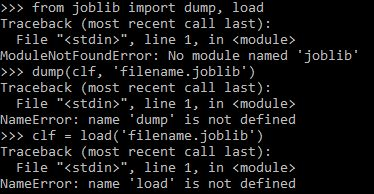
\includegraphics[width=0.75\textwidth]{figures/huda/18.JPG}}\caption{Hasil Tampilan Error.}\end{figure}
\subsubsection{Tuliskan Kode Eror dan Jenis Erornya}
\begin{itemize}
\item \begin{verbatim}from joblib import dump, load\end{verbatim} (Kode baris pertama)
\subitem \begin{verbatim}
Traceback(most recent call last):
 File "<stdin>", line 1, in<module>
ModuleNotFoundError: No module named 'joblib'
\end{verbatim} (Errornya)
\item \begin{verbatim}dump(clf, 'filename.joblib')\end{verbatim} (Kode baris kedua)
\subitem \begin{verbatim}
Traceback(most recent call last):
 File "<stdin>", line 1, in<module>
NameError: name 'dump' is not defined
\end{verbatim} (Errornya)
\item \begin{verbatim}clf = load('filename.joblib')\end{verbatim} (Kode baris ketiga)
\subitem \begin{verbatim}
Traceback(most recent call last):
 File "<stdin>", line 1, in<module>
NameError: name 'load' is not defined
\end{verbatim} (Errornya)
\end{itemize}
\subsubsection{Solusi Pemecahan Masalah Error}
\begin{enumerate}
\item Pada masalah error sebelumnya itu dikarenakan kita belum mempunyai packaged joblib. Jadi solusinya yaitu dengan cara menginstall terlebih dahulu packaged joblibnya setelah itu baru perintah tersebut dapat dijalankan seperti pada gambar 1.2 dan 1.3
\begin{figure}[ht]\centerline{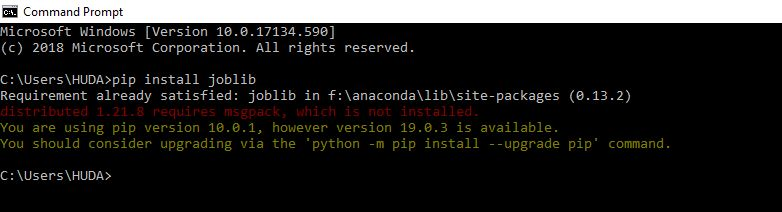
\includegraphics[width=0.75\textwidth]{figures/huda/33.JPG}}\caption{Hasil Tampilan Install joblib.}\end{figure}
\begin{figure}[ht]\centerline{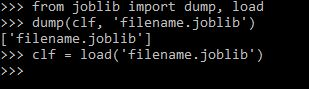
\includegraphics[width=0.75\textwidth]{figures/huda/32.JPG}}\caption{Hasil Tampilan Uji coba perintah joblib.}\end{figure}
\end{enumerate}

\begin{figure}[ht]\centerline{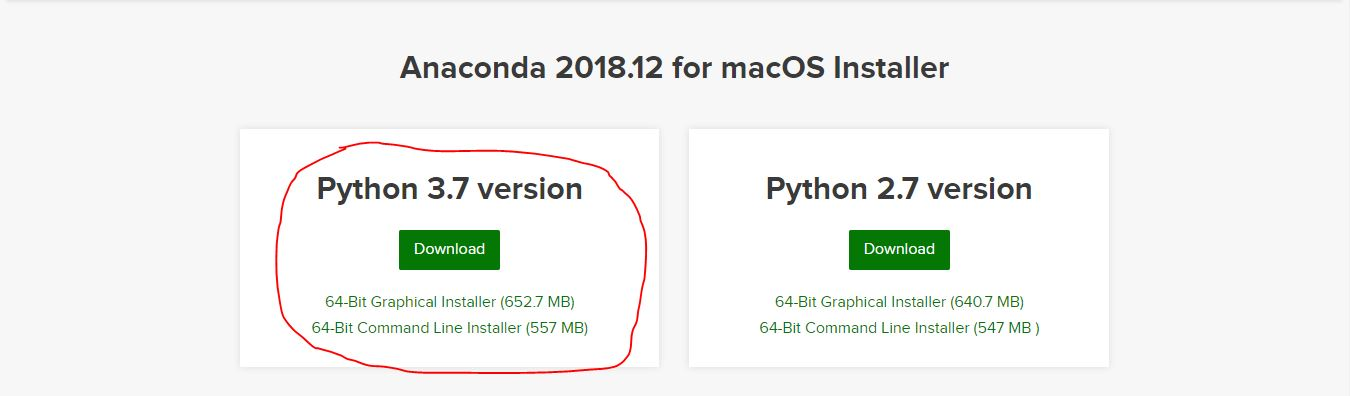
\includegraphics[width=1\textwidth]{figures/huda/1.JPG}}\caption{Download Anaconda.}\end{figure}
\begin{figure}[ht]\centerline{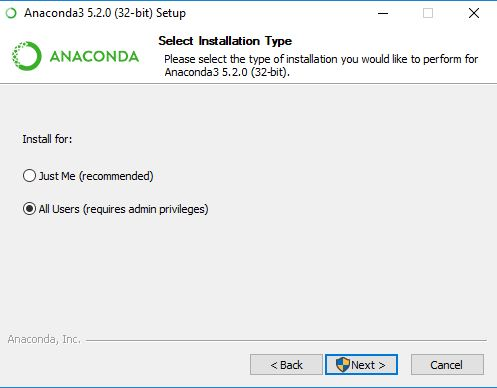
\includegraphics[width=0.75\textwidth]{figures/huda/2.JPG}}\caption{Langkah pertama instalasi anaconda.}\end{figure}
\begin{figure}[ht]\centerline{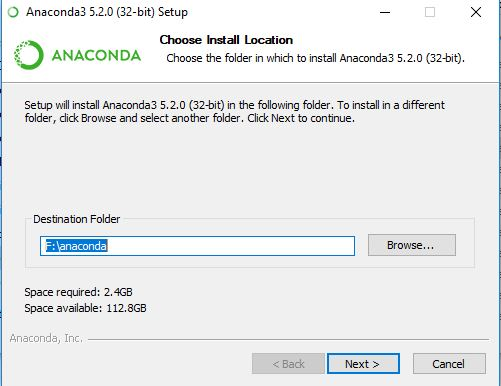
\includegraphics[width=0.75\textwidth]{figures/huda/3.JPG}}\caption{Langkah kedua instalasi anaconda.}\end{figure}
\begin{figure}[ht]\centerline{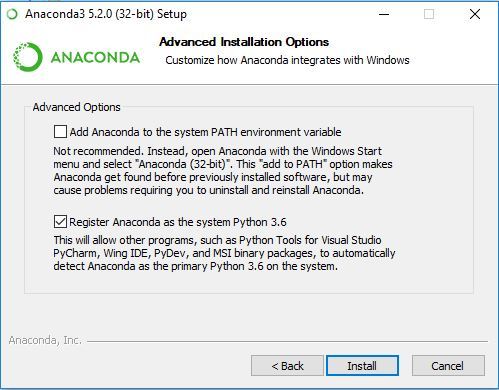
\includegraphics[width=0.75\textwidth]{figures/huda/4.JPG}}\caption{Langkah ketiga instalasi anaconda.}\end{figure}
\begin{figure}[ht]\centerline{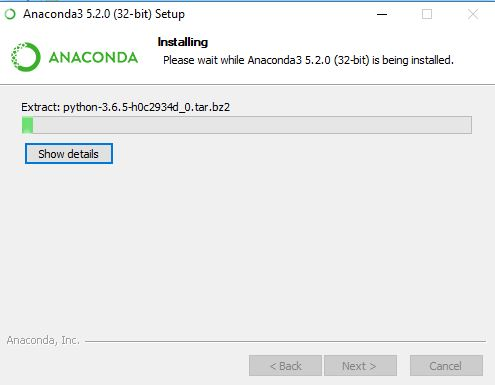
\includegraphics[width=0.75\textwidth]{figures/huda/5.JPG}}\caption{Langkah terakhir instalasi anaconda.}\end{figure}
\begin{figure}[ht]\centerline{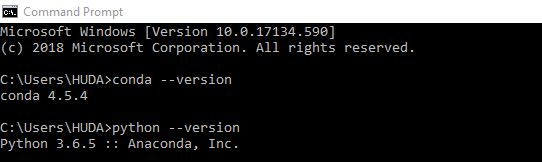
\includegraphics[width=0.75\textwidth]{figures/huda/6.JPG}}\caption{Langkah pertama instalasi scikit pada CMD.}\end{figure}
\begin{figure}[ht]\centerline{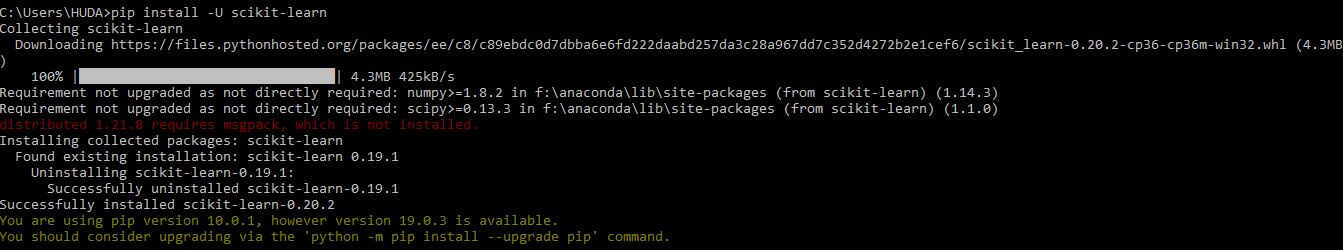
\includegraphics[width=0.75\textwidth]{figures/huda/7.JPG}}\caption{Langkah kedua instalasi scikit pada CMD.}\end{figure}
\begin{figure}[ht]\centerline{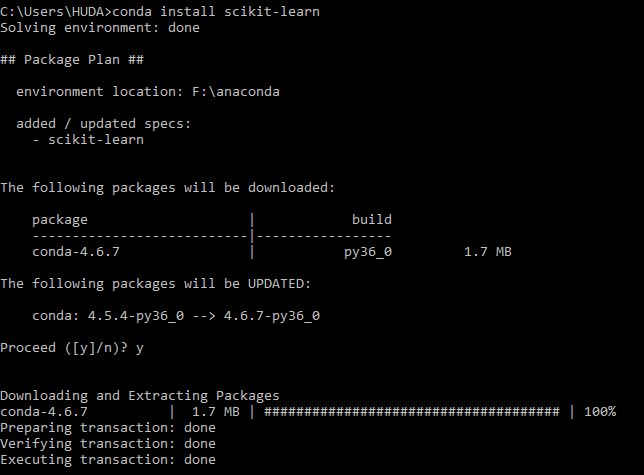
\includegraphics[width=0.75\textwidth]{figures/huda/8.JPG}}\caption{Langkah ketiga instalasi scikit pada CMD.}\end{figure}
\begin{figure}[ht]\centerline{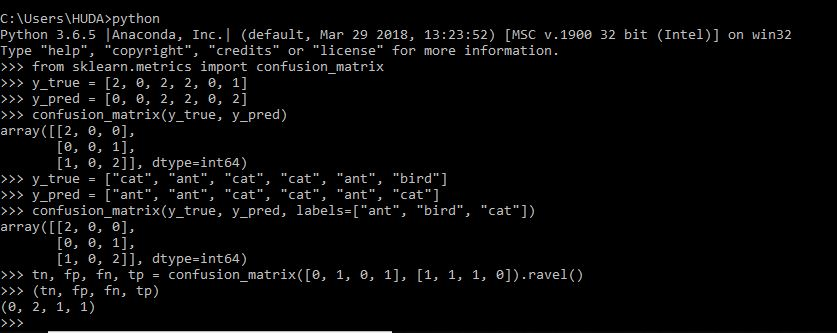
\includegraphics[width=0.75\textwidth]{figures/huda/9.JPG}}\caption{Langkah compile code pada python anaconda.}\end{figure}
\begin{figure}[ht]\centerline{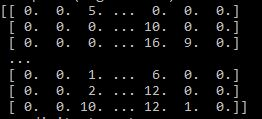
\includegraphics[width=0.75\textwidth]{figures/huda/10.JPG}}\caption{Hasil Tampilan 1.}\end{figure}
\begin{figure}[ht]\centerline{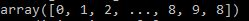
\includegraphics[width=0.75\textwidth]{figures/huda/11.JPG}}\caption{Hasil Tampilan 2.}\end{figure}
\begin{figure}[ht]\centerline{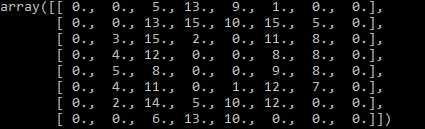
\includegraphics[width=0.75\textwidth]{figures/huda/12.JPG}}\caption{Hasil Tampilan 3.}\end{figure}
\begin{figure}[ht]\centerline{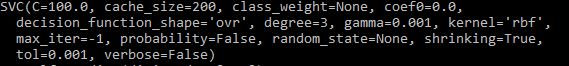
\includegraphics[width=0.75\textwidth]{figures/huda/13.JPG}}\caption{Hasil Tampilan 4.}\end{figure}
\begin{figure}[ht]\centerline{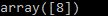
\includegraphics[width=0.75\textwidth]{figures/huda/14.JPG}}\caption{Hasil Tampilan 5.}\end{figure}
\begin{figure}[ht]\centerline{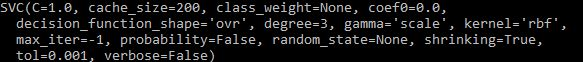
\includegraphics[width=0.75\textwidth]{figures/huda/15.JPG}}\caption{Hasil Tampilan 6.}\end{figure}
\begin{figure}[ht]\centerline{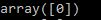
\includegraphics[width=0.75\textwidth]{figures/huda/16.JPG}}\caption{Hasil Tampilan 7.}\end{figure}
\begin{figure}[ht]\centerline{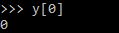
\includegraphics[width=0.75\textwidth]{figures/huda/17.JPG}}\caption{Hasil Tampilan 8.}\end{figure}
\begin{figure}[ht]\centerline{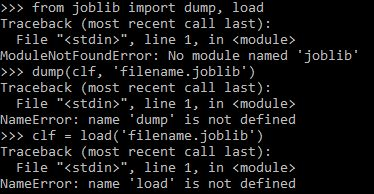
\includegraphics[width=0.75\textwidth]{figures/huda/18.JPG}}\caption{Hasil Tampilan 9.}\end{figure}
\begin{figure}[ht]\centerline{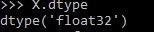
\includegraphics[width=0.75\textwidth]{figures/huda/19.JPG}}\caption{Hasil Tampilan 10.}\end{figure}
\begin{figure}[ht]\centerline{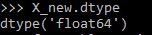
\includegraphics[width=0.75\textwidth]{figures/huda/20.JPG}}\caption{Hasil Tampilan 11.}\end{figure}
\begin{figure}[ht]\centerline{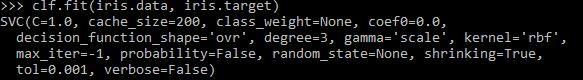
\includegraphics[width=0.75\textwidth]{figures/huda/21.JPG}}\caption{Hasil Tampilan 12.}\end{figure}
\begin{figure}[ht]\centerline{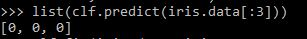
\includegraphics[width=0.75\textwidth]{figures/huda/22.JPG}}\caption{Hasil Tampilan 13.}\end{figure}
\begin{figure}[ht]\centerline{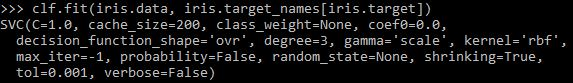
\includegraphics[width=0.75\textwidth]{figures/huda/23.JPG}}\caption{Hasil Tampilan 14.}\end{figure}
\begin{figure}[ht]\centerline{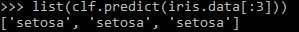
\includegraphics[width=0.75\textwidth]{figures/huda/24.JPG}}\caption{Hasil Tampilan 15.}\end{figure}
\begin{figure}[ht]\centerline{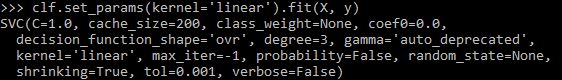
\includegraphics[width=0.75\textwidth]{figures/huda/25.JPG}}\caption{Hasil Tampilan 16.}\end{figure}
\begin{figure}[ht]\centerline{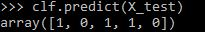
\includegraphics[width=0.75\textwidth]{figures/huda/26.JPG}}\caption{Hasil Tampilan 17.}\end{figure}
\begin{figure}[ht]\centerline{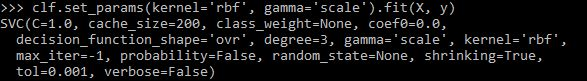
\includegraphics[width=0.75\textwidth]{figures/huda/27.JPG}}\caption{Hasil Tampilan 18.}\end{figure}
\begin{figure}[ht]\centerline{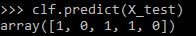
\includegraphics[width=0.75\textwidth]{figures/huda/28.JPG}}\caption{Hasil Tampilan 19.}\end{figure}
\begin{figure}[ht]\centerline{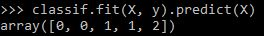
\includegraphics[width=0.75\textwidth]{figures/huda/29.JPG}}\caption{Hasil Tampilan 20.}\end{figure}
\begin{figure}[ht]\centerline{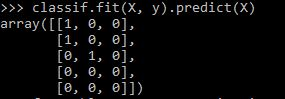
\includegraphics[width=0.75\textwidth]{figures/huda/30.JPG}}\caption{Hasil Tampilan 21.}\end{figure}
\begin{figure}[ht]\centerline{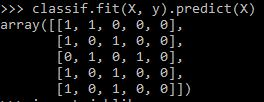
\includegraphics[width=0.75\textwidth]{figures/huda/31.JPG}}\caption{Hasil Tampilan 22.}\end{figure}

=======
<<<<<<< HEAD
\section{Cokro Edi Prawiro/1164069}
\subsection{Praktek teori penunjang}
\begin{enumerate}
\item
Kecerdasan Buatan \textit{Artificial Intelligence} adalah suatu cabang dalam bidang sains komputer yang mengkaji bagaimana untuk melengkapi sebuah komputer dengan kemampuan atau kepintaran saperti manusia. Komputer tersebut di harapkan dapat belajar sendiri dengan cara mengumpulkan data-data yang diterimanya, yang berguna sebagai parameter untuk memecahkan masalah. Jadi kecerdasan buatan merupakan kecerdasan yang di program dalam koputer untuk memecahkan masalah secara tepat dan cepat atau untuk memberikan kemungkinan keberhasilan dan kegagalan pada solusi dari suatu masalah.\par
Adapun kecerdasan buatan menurut para ahli adalah sebagai berikut :
\begin{itemize}
\item 
Kecerdasan Buatan merupakan Kawasan penelitian, aplikasi dan intruksi yang terkait dengan pemerograman komputer untuk melakukan sesuatu hal yang dalam pandangan manusia adalah cerdas (H. A. Simon[1997]).
\item 
Kecerdasan buatan adalah bidang studi yang berhubungan dengan penangkapan, pemodelanm, dan penyimpanan kecerdasan manusia dalam sebuah sistem teknologi sehingga sistem tersebut dapat menfasilitasi proses pengambilan keputusan yang biasanya dilakukan oleh manusia (Haag dan keen[1996]).
\end{itemize}
Sejarah dan Perkembangan Kecerdasan Buatan.\\
ketika \textit{Rene Descartes} mengemukakan gagasan yang menjadi cikal bakal kecerdasan buatan pada abad 17 mengemukakan bahwa hewan bukan apa-apa melainkan hanya mesin yang rumit yang dilanjutkan oleh \textit{Belaise Pascal} yang telah menciptakan mesin penghitung digital mekanis pertama pada tahun 1642. Lalu pada abad 19 \textit{Charles Babbage} dan\textit{Ada lovelace}  bekerja sama membuat mesin penghitung mekanis yang dapat di program.\par
Perkembangan kecerdasan buatan inipun terus berlanjut,\textit{ Bertrand Russell} dan\textit{ Alferd North Whithead} menerbitkan \textit{mathematica}, yang merombak logika formal. Setelah itu dilanjutkan dengan penemuan oleh \textit{ Warren McCulloch} dan \textit{ Walter Pitts} menerbitkan “Kalkulus Logis Gagasan yang tetap ada dalam Aktivitas” pada 1943 yang meletakan pondasi awal berupa jaringan syaraf 
Kemudian pada tahun 1950-an adalah periode awal usaha aktif kecerdasan buatan. Progam Kecerdasan buatan pertama yang bekerja di ciptakan pada tahun 1951 untuk menjalankan mesin Ferranti Mark I di University of Manchester (UK) yaitu sebuah program permainan naskah yang ditulis oleh \textit{Christoper Strachey} dan program permainan catur yang ditulis oleh \textit{Dietric Prinz}. Kemudian pada konferensi pertama tahun 1956  \textit{John McCarthy} mengemukakan istilah “kecerdasan buatan” kemudian dia juga menemukan bahasa pemerograman lips. \textit{Joseph Weizenbaum}  menciptakan ELIZA, sebuah chatterbot yang menerapkan psikoterapi Rogerian.\par
Selama rentang waktu tahun 1960-an dan 1970-an, \textit{Joel Moses}  mendemonstrasikan kekuatan pertimbangan simbolis untuk mengintegrasikan masalah di dalam program Macsyma, yang merupakan program yang pertamakali sukses dalam bidang matematika. Kemudian pada tahun 1980-an industry kecerdasan buatan ini berkembang walu sudah di mulai pada tahun 1970-an Evolusi kecerdasan buatan berjalan dalam dua jalur yang berbeda yaitu meniru proses berpikir manusia untuk menyelesaikan masalah umum. Kedua mengkombinasikan pemikiran terbaik para ahli pada sepotong software yang dirancang untuk memecahkan persolalan yang spesifik. 

\item
Supervised learning adalah sebuah pendekatan dengan syarat sudah terdapat data yang dilatih kemudian harus terdapat variable yang ditargetkan sehingga tujuan dari pendekatan ini adalah pengelompokan data terhadap data yang telah ada. Ciri khas dari Supervised learning yaitu terdapat label atau nama kelas pada data latih (supervisi) dan data baru di klasifikasikan berdasarkan data latih. Data latih sikelompokan berdasarkan ukuran kemiripan pada suatu kelas. Berdasarkan keluaran dari fungsi, Supervised learning dibagi menjadi 2, regresi dan klasifikasi. Regresi terjadi jika output dari fungsi merupakan nilai yang kontinyu, sedangkan klasifikasi terjadi jika keluaran dari fungsi adalah nilai tertentu dari suatu atribut (tidak kontinyu). Tujuan dari Supervised learning adalah untuk memprediksi nilai dari fungsi untuk sebuah data masukanyang sah setelah melihat sejumlah data latih\cite{februariyanti2012klasifikasi}.\\
Adapun pengertian klasifikasi dan regresi adalah sebagai berikut :
\begin{itemize}
\item
Klasifikasi merupakan pengelompokan berdasarkan parameter tertentu yang tidak konstan contoh pada mahluk hidup yaitu persamaan ciri cara hidup dan tempat hidup.
\item
Regresi yaitu pengeluaran nilai output yang konstan jika dipicu dengan parameter tertentu biasanya regresi disini berbentuk regresi linier. Regresi linier yaitu metode statistika yang digunakan untuk membentuk model hubungan antara variabel terikat(dependen,respon,Y) dengan satu atau lebih variabel bebas(independent, prdiktor, X). Apabila banyaknya variabel bebas hanya ada satu, disebut sebagai regresi linier sederhana, sedangkan apabila terdapat lebih dari satu variabel bebas, disebut sebagai regresi linier berganda \cite{kurniawan2008regresi}.
\end{itemize}
unsupervised learning adalah pendekatan yang tidak memerlukan data latih atau data training untuk melakukan prediksi atau klasifikasi. Berdasarkan model secara matematisnya, algoritma ini tidak memiliki target variabel. Tujuan dari algoritma ini yaitu pengelompokan objek yang memiliki kesamaan atau hampirsama dalam satu cakupan wilayah tertentu. Kemudian pada unsupervised learning tidak terdapat label atau nama kelas pada data latih.
Kemudian dataset merupakan objek yang menggambarkan data itu sendiri dan relasinya di memory. Struktur datanya mirip dengan struktur data di basisdata. Jadi strikturnya terdiri atas baris kolon dan juga ada sejenis relasi data. Pada dataset terdiri bagian bagian yaitu tranning set dan Testing set.
Adapun pengertian dari tranning set dan Testing set adalah sebagai berikut :
\begin{itemize}
\item
Training set adalah bagian dari dataset itu sendiri yang dilatih untuk membuat prediksi atau algoritma mesin learning lainnya sesuai keinginan atau tujuan data itu dibuat.
\item
Testing set adalah bagian dari dataset yang di tes atau diujicoba untuk melihat keakuratannya dengan katalain melihat peformanya.
\end{itemize}
\end{enumerate}

\subsection{Instalisasi}\par
Pada proses instalisasi ini langkah pertama yaitu mengakses website scikit dengan mengakses link berikut  https://scikit-learn.org/stable/tutorial/basic/tutorial.html maka hsilnya dapat dilihat pada gambar \ref{sc} kemudian setelah itu klik button installation maka akan muncul tampilan yang dapat dilihat pada gambar \ref{sc1}.
\begin{figure}[ht]
      \centerline{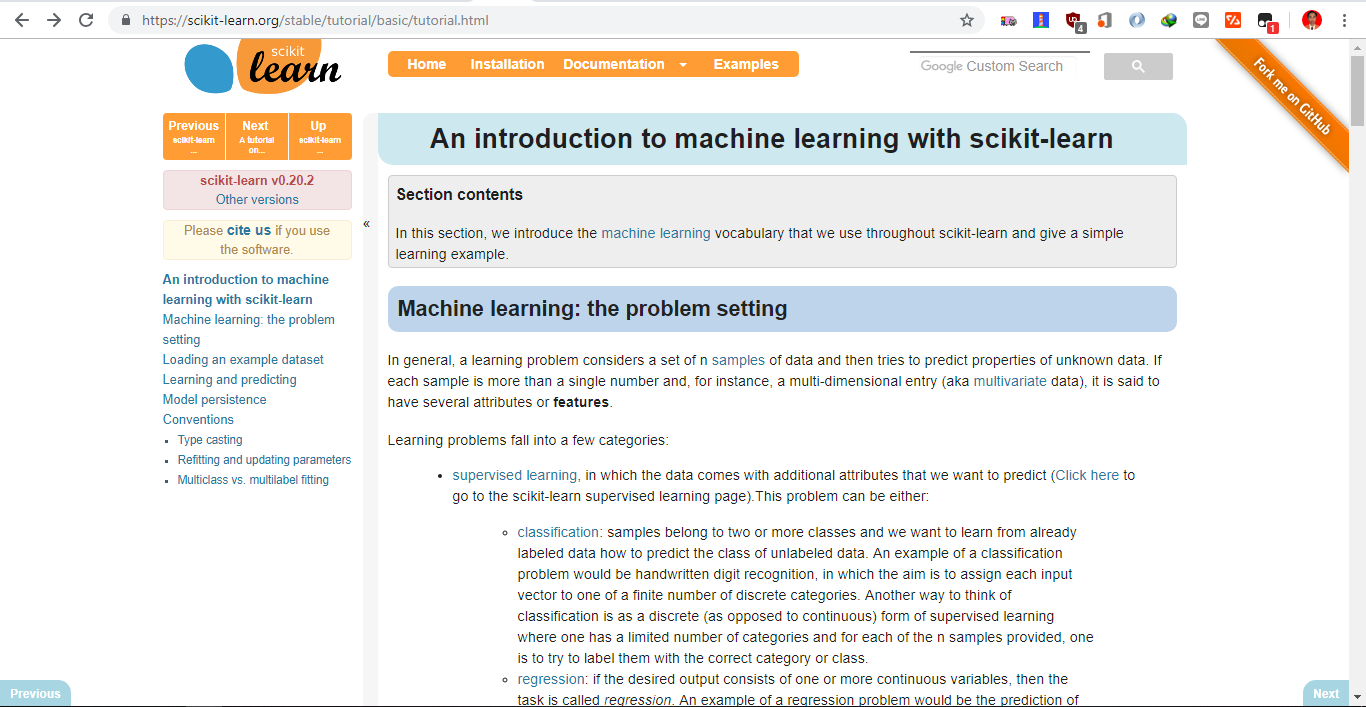
\includegraphics[width=1\textwidth]
      {figures/sc}}
      \caption{Tampilan website Scikit 1.}
      \label{sc}
      \end{figure}
\begin{figure}[ht]
      \centerline{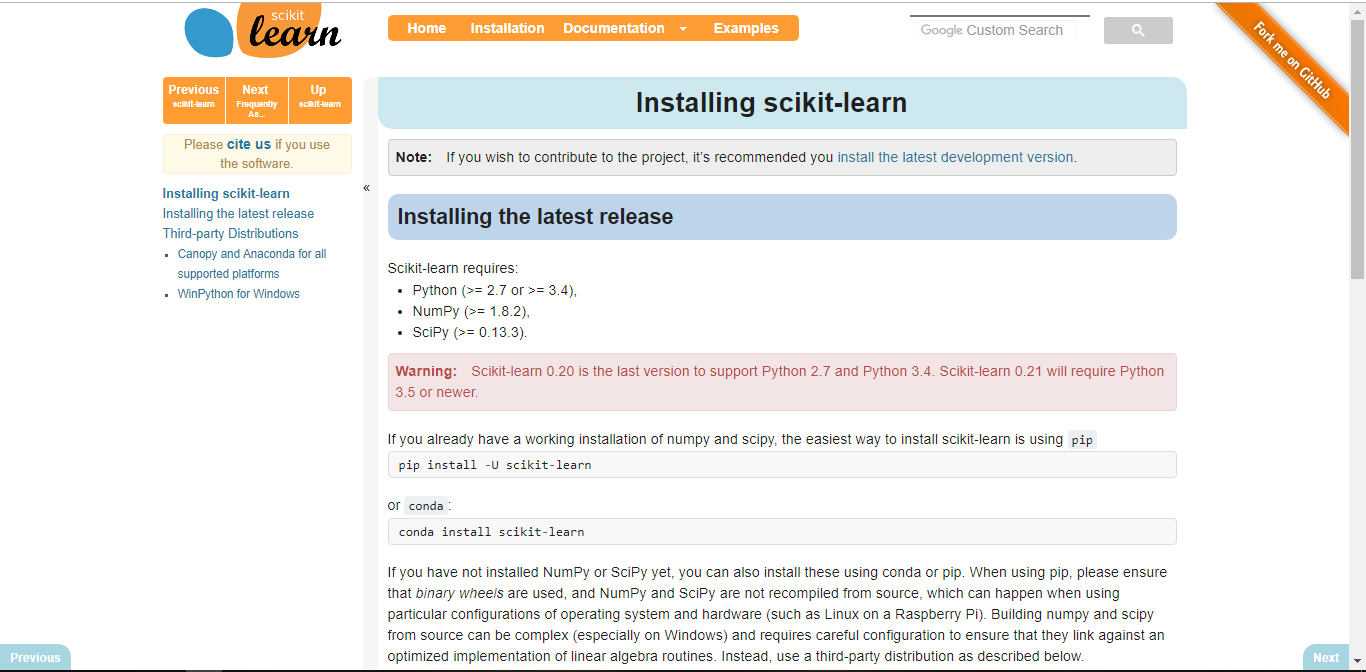
\includegraphics[width=1\textwidth]
      {figures/sc1}}
      \caption{Tampilan website Scikit 2.}
      \label{sc1}
      \end{figure}
\begin{enumerate}
\item 
cara instalisasi Instalasi library scikit dari anaconda langkah pertama instal terlebih dahulu anacondanya dikarenakan anaconda sudah include dengan python maka codingan python dapat digunakan di anaconda dan ketika diperikas versinya maka akan muncul tampilan seperti Gambar \ref{c}

kemudian pada cmd administrator install library sikic dengan cara memasukan codingan pip install -U scikit-learn maka hasilnya seperti seperti pada gambar \ref{c1} berikut.

setelah itu masukan kembali perintah berikut di cmd conda install scikit-learn jika hasilnya seperti pada gambar \ref{c2} maka librari sikic telah teristal dan siap untuk di gunakan.

kemudian untuk mencobanya tuliskan perintah python pada cmd lalu masukan codingan print("Hello Anaconda!") maka hasilnya terlihat seperti gambar \ref{c3} codingan print("Hello Anaconda!") yaitu berfungsi mencetak nilai yang ada di dalam kurung dan di antara kutip.


\item
cara mencoba dataset yaitu dengan cara memasukan perintah berikut pada cmd seperti pada gambar \ref{c4} 

\begin{itemize}
\item
pada codingan from sklearn import datasets menjelaskan inport librari dataset dari librari sikic pada gambar \ref{c4}
\item
pada codingan iris = datasets.load iris iris beearti parameter atau acuan bernama iris kemudian di load ke dalam dataset sebagai perbandingan kalau daram diagram iris bisa disebut X nya pada gambar \ref{c4}
\item 
pada codingan digits = datasets.load digits digits berarti parameter hampir mirip seperti iris tadi namun digits merupakan kebalikannya kalau di dalam diagaram dia bernilai Y pada gambar \ref{c4}
\item
kemudian pada codingan print(digits.data) yaitu mencetak data digits yang di bandingkan dengan data iris pada gambar \ref{c4}
\item 
pada codingan print(iris.data) yaitu mencetak data iris yang dibandingkan dengan data digits pada gambar \ref{c4}
\end{itemize}
\item
Mencoba Learning and Predicting\par
Pada kasus ini dataset digit digunakan untuk memprediksi yang mana telah di berikan gambar untuk mewakili sampel masing-masing dari 10 kelas yang dimulai dari digit nol hingga sembilan yang digunakan untuk memprediksi sampel yang tidak terlihat untuk lebih jelasnya dapat di praktikan codingan berikut ini.

\begin{verbatim}
>>> from sklearn import datasets 
\end{verbatim}
pada baris ini dapat diartikan bahwa librari sklearn mengimport package dataset
\begin{verbatim}
>>> iris = datasets.load_iris() 
\end{verbatim}
pada baris ini dimasukan parameter iris yang di sandingkan dengan dataset load sehingga iris berisi nilai dataset
\begin{verbatim}
>>> digits = datasets.load_digits()
\end{verbatim}
pada baris ini dimasukan parameter digits yang di sandingkan dengan dataset load sehingga digits berisi nilai dataset
\begin{verbatim}
>>> from sklearn import svm
\end{verbatim}
pada baris ini  librari sklearn mengimport package svm
\begin{verbatim}
>>> clf = svm.SVC(gamma=0.0001, C=100.)
\end{verbatim}
pada codingan diatas dibuat variabel clf yang di isi dengan nilai svm dengan nilai gama 0.0001 dan 100.
\begin{verbatim}
>>> clf.fit(digits.data[:-1], digits.target[:-1])
\end{verbatim}
pada codingan clf di implementasikan dengan perintah fit
\begin{verbatim}
SVC(C=100.0, cache_size=200, class_weight=None, coef0=0.0,
  decision_function_shape='ovr', degree=3, gamma=0.0001, kernel='rbf',
  max_iter=-1, probability=False, random_state=None, shrinking=True,
  tol=0.001, verbose=False)
\end{verbatim}
yang hasilnya seperti codingan diatas yang menjabarkan isi dari SVC itu sendiri.
\begin{verbatim}
>>> clf.predict(digits.data[-1:])
array([8])
>>>
\end{verbatim}
kemudain pada codingan diatas digunakan printah predic yang merupakan printah untuk mengimplementasikan method digits.
\item
Mencoba model pertistence\par 
model pertistence yaitu model yang digunakan untuk mengolah data sehingga data tersebut konstan atau konsisten terhadap parameter tertentu contoh pada codingan di bagawah nilai y akan konstan di nol walaupuntelah di isi nilai lebih dari nol.
\begin{verbatim}
>>> from sklearn import svm
\end{verbatim}
pada baris ini  librari sklearn mengimport package svm.
\begin{verbatim}
>>> from sklearn import datasets
\end{verbatim}
pada baris ini  librari sklearn mengimport package datasets.
\begin{verbatim}
>>> clf = svm.SVC(gamma='scale')
\end{verbatim}
pada codingan diatas dibuat variabel clf yang di isi dengan nilai svm dengan gamma sama dengan scale.
\begin{verbatim}
>>> iris = datasets.load_iris()
\end{verbatim}
pada baris ini dimasukan parameter iris yang di sandingkan dengan dataset load sehingga iris berisi nilai dataset.
\begin{verbatim}
>>> X, y = iris.data, iris.target
\end{verbatim}
pada codingan diatas X berisi nilai iris.data dan y berisi nilai iris.target.
\begin{verbatim}
>>> clf.fit(X, y)
\end{verbatim}
method clf di implementasikan dengan perintah fit dengan X, y sebagai nilai untuk implementasinya.
\begin{verbatim}
SVC(C=1.0, cache_size=200, class_weight=None, coef0=0.0,
  decision_function_shape='ovr', degree=3, gamma='scale', kernel='rbf',
  max_iter=-1, probability=False, random_state=None, shrinking=True,
  tol=0.001, verbose=False)
\end{verbatim}
maka hasilnya penjabaran dari SVC seperti codingan diatas.
\begin{verbatim}
>>> import pickle
\end{verbatim}
mengimport library atau package pickle.
\begin{verbatim}
>>> s = pickle.dumps(clf)
\end{verbatim}
kemudian di buat variabel s yang di load oleh package pickle dengan di isi nilai clf.
\begin{verbatim}
>>> clf2 = pickle.loads(s)
\end{verbatim}
setelah itu pada codingan diatas dibuat lagi variabel clf2 kemudian di load pickle.
\begin{verbatim}
>>> clf2.predict(X[0:1])
\end{verbatim}
kemudian variabel clf2 di implementasikan dengan parameter X dengan nilai 0 berbanding 1maka hasilnya nilainya array bernilai nol dan y bernialai nol.
\begin{verbatim}
array([0])
>>> y[0]
0
\end{verbatim}
\item
mencoba conventions
convenstiions merupakan aturan aturan dasar atau kesepakatan kesepakatan dalam pemerograman sikit python dan anaconda berikut merupakan jenis-jenis codingan conventions :
\begin{itemize}
\item
Type casting yaitu tipe pelemparan parameter atau variabel kedalam variabel baru.
\begin{verbatim}
>>> import numpy as np
\end{verbatim}
codingan diatas yaitu import librari numpy yang di inisialisasi menjadi np
\begin{verbatim}
>>> from sklearn import random_projection
\end{verbatim}
import librari random\_projection
\begin{verbatim}
>>> rng = np.random.RandomState(0)
\end{verbatim}
membuat variabel baru dengan nama rng dengan nilai random
\begin{verbatim}
>>> X = rng.rand(10, 2000)
\end{verbatim}
memasukan nilai rng kedalam variabel X dengan rad nilai 10 sampai 2000
\begin{verbatim}
>>> X = np.array(X, dtype='float32')
\end{verbatim}
menambahkan nilai np berupa array yaitu X dan float 32 
\begin{verbatim}
>>> X.dtype
dtype('float32')
\end{verbatim}
X.dtype di running menghasilkan nilai dtype float
\begin{verbatim}
>>> transformer = random_projection.GaussianRandomProjection()
\end{verbatim}
membuat variabel transformer dengan nilai random
\begin{verbatim}
>>> X_new = transformer.fit_transform(X)
\end{verbatim}
membuat variabel X\_new dan di isi nilai transformer kemudian di implementasikan 
\begin{verbatim}
>>> X_new.dtype
\end{verbatim}
merunning variabel X\_new
\begin{verbatim}
dtype('float64')
\end{verbatim}
hasil running X\_new


\begin{verbatim}
>>> from sklearn import datasets
\end{verbatim}
mengimport library dataset
\begin{verbatim}
>>> from sklearn.svm import SVC
\end{verbatim}
mengimport library SVC
\begin{verbatim}
>>> iris = datasets.load_iris()
\end{verbatim}
membuat variabel iris dengan nilai load dataset
\begin{verbatim}
>>> clf = SVC(gamma='scale')
\end{verbatim}
membuat variabel clf bernilai SVC dengan gamma menggunakan nilai sekala
\begin{verbatim}
>>> clf.fit(iris.data, iris.target)
\end{verbatim}
merunning variabel atau method clf dengan isian nilai iris data dan iris target
\begin{verbatim}
SVC(C=1.0, cache_size=200, class_weight=None, coef0=0.0,
  decision_function_shape='ovr', degree=3, gamma='scale', kernel='rbf',
  max_iter=-1, probability=False, random_state=None, shrinking=True,
  tol=0.001, verbose=False)
\end{verbatim}
detail hasil runing clf 
\begin{verbatim}
>>> list(clf.predict(iris.data[:3]))
[0, 0, 0]
\end{verbatim}
memunculkan detail atau lis sebanyak tiga nilai
\begin{verbatim}
>>> clf.fit(iris.data, iris.target_names[iris.target])
\end{verbatim}
merunning kembali clf dengan nilai iris data, iris target name
\begin{verbatim}
SVC(C=1.0, cache_size=200, class_weight=None, coef0=0.0,
  decision_function_shape='ovr', degree=3, gamma='scale', kernel='rbf',
  max_iter=-1, probability=False, random_state=None, shrinking=True,
  tol=0.001, verbose=False)
\end{verbatim}
hasil dari running clf
\begin{verbatim}
>>> list(clf.predict(iris.data[:3]))
['setosa', 'setosa', 'setosa']
\end{verbatim}
memunculkan tiga nilai yang telah dilempar dari SVC
\item
Refitting and updating parameters atau pengisian ulang atau memperbagarui paramater merupakan cara untuk merubah nilai dari sebuah parameter contoh nilai x adalah 10 jika di perbaharui bisa menjadi 15 begitu juga dalam codiangan berikut hal ini dapat dilakukan untuk lebih jelasnya dabat dilihat codingan dibawah ini :
\begin{verbatim}
>>> import numpy as np
\end{verbatim}
codingan diatas yaitu import librari numpy yang di inisialisasi menjadi np
\begin{verbatim}
>>> from sklearn.svm import SVC
\end{verbatim}
mengimport library SVC
\begin{verbatim}
>>> rng = np.random.RandomState(0).
\end{verbatim}
membuat variabel baru dengan nama rng dengan nilai random.
\begin{verbatim}
>>> X = rng.rand(100, 10)
\end{verbatim}
paramater X dengan nilai dari variabel rng dan rad dari 100 sampai 10.
\begin{verbatim}
>>> y = rng.binomial(1, 0.5, 100)
\end{verbatim}
parameter y dengan nilai rng binominal dari 1 0,5 sampai 100.
\begin{verbatim}
>>> X_test = rng.rand(5, 10)
\end{verbatim}
parameter X\_test dengan nilai rng dan rad dari 5 ke 10
\begin{verbatim}
>>> clf = SVC()
\end{verbatim}
parameter clf bernilai SVC
\begin{verbatim}
>>> clf.set_params(kernel='linear').fit(X, y)
\end{verbatim}
parameter clf di set dengan mengkompile atau mengekstrak nilai X dan y dengan kernel linear.
\begin{verbatim}
SVC(C=1.0, cache_size=200, class_weight=None, coef0=0.0,
  decision_function_shape='ovr', degree=3, gamma='auto_deprecated',
  kernel='linear', max_iter=-1, probability=False, random_state=None,
  shrinking=True, tol=0.001, verbose=False)
\end{verbatim}
penjabaran nilai SVC hasul running CLF
\begin{verbatim}
>>> clf.predict(X_test)
array([1, 0, 1, 1, 0])
\end{verbatim}
meranning clf dengan nilai X\_test
\begin{verbatim}
>>> clf.set_params(kernel='rbf', gamma='scale').fit(X, y)
\end{verbatim}
parameter clf di set dengan kernel rbf dan gama skala dan mengkompile nilai X dan y.
\begin{verbatim}
SVC(C=1.0, cache_size=200, class_weight=None, coef0=0.0,
  decision_function_shape='ovr', degree=3, gamma='scale', kernel='rbf',
  max_iter=-1, probability=False, random_state=None, shrinking=True,
  tol=0.001, verbose=False)
\end{verbatim}
penjabaran nilai SVC hasul running CLF
\begin{verbatim}
>>> clf.predict(X_test)
array([1, 0, 1, 1, 0])
\end{verbatim}
Hasil dari  running clf.
\item
Multiclass vs. multilabel fitting
perbandingan antara bnyak klass dan pelabelan yang tepat berikut merupakan codingannya.
\begin{verbatim}
>>> from sklearn.svm import SVC
\end{verbatim}
mengimport library SVC
\begin{verbatim}
>>> from sklearn.multiclass import OneVsRestClassifier
\end{verbatim}
memasukan librari OneVsRestClassifier dengan kondisi multi class.
\begin{verbatim} 
>>> from sklearn.preprocessing import LabelBinarizer
\end{verbatim}
memasukan librari  LabelBinarizer
\begin{verbatim}
>>> X = [[1, 2], [2, 4], [4, 5], [3, 2], [3, 1]]
\end{verbatim}
pemberian nilai pada parameter X
\begin{verbatim}
>>> y = [0, 0, 1, 1, 2]
\end{verbatim}
pemberian nilai pada parameter y
\begin{verbatim}
>>> classif = OneVsRestClassifier(estimator=SVC(gamma='scale',
... random_state=0))
\end{verbatim}
opsi untuk class dengan ketentuan estimator SVC gamma berbentuk skala dan random (acak).
\begin{verbatim}
>>> classif.fit(X, y).predict(X)
array([0, 0, 1, 1, 2])
\end{verbatim}
hasil array dari running classif
\begin{verbatim}
>>> y = LabelBinarizer().fit_transform(y)
\end{verbatim}
memberikan niilai pada parameter y
\begin{verbatim}
>>> classif.fit(X, y).predict(X)
array([[1, 0, 0],
       [1, 0, 0],
       [0, 1, 0],
       [0, 0, 0],
       [0, 0, 0]])
\end{verbatim}
hasil running classif 
\begin{verbatim}
>>> from sklearn.preprocessing import MultiLabelBinarizer
\end{verbatim}
import librari multi label
\begin{verbatim}
>>> y = [[0, 1], [0, 2], [1, 3], [0, 2, 3], [2, 4]]
\end{verbatim}
memberikan nilai pada parameter y
\begin{verbatim}
>>> y = MultiLabelBinarizer().fit_transform(y)
\end{verbatim}
membuat parameter y menjadi multi label.
\begin{verbatim}
>>> classif.fit(X, y).predict(X)
=======

\section{Fathi Rabbani / 1164074}
\subsection{Teori}
\begin{enumerate}
\item
Sejarah dan Perkembangan Kecerdasan Buatan
\subitem
Sejarah dari sebuah Artificial Intelligence atau dalam Bahasa indonesianya diterjemahkan sebagai Kecerdasan Buatan adalah sebuah usaha untuk dapat memodelkan sebuah mesin agar dapat berfikir dan menirukan tingkah laku dan cara berfikir manusia, ada beberapa jenis dari kecerdasan buatan, yaitu :

\begin{itemize}
\item
Symbol Manipulating AI
\item
Nueral AI
\item
Neural Network
\end{itemize}
\subitem
Peneliti yang selalu disebutkan sebagai Bapak AI adalah Jhon McCharty  merupakan seorang dosen yang mengenalkan Kecerdasan Buatan kepada 2 lembaga penelitian hebat, yaitu Stanford Artificial Intelligence Laboratory dan MIT Artificial Intelligence Laboratory.
\subitem
Sedangkan perkembangan kecerdasan buatan saat ini sudah mencapai tahap dimana manusia mulai membuat sebuah robot yang dapat menirukan hampir 90 persen dari keseharian mereka, mulai dari bidang kesehatan, koki, pabrik, kantoran, hingga sebuah robot yang bertugas sebagai seorang pelayan di sebuah restoran. Dan dubai sebagai pengguna mobil tanpa pengemudi yang menerapkan AI dengan menggunakan data wilayah serta jarak kendaraan dengan pingir jalan.
\item
Definisi Supervised, Unsupervised Learning, Klasifikasi, Regresi serta Data, Training, Testing Set
\begin{itemize}
\item
Supervised learning merupakan sebuah pendekatan AI dengan latihan yang sudah dilakukan dengan sebuah data yang lengkap, dan memiliki variable yang dapat digunakan sebagai target sehingga dapat menujukan data agar menjadi kelompok dari sebuah data menjadi kelompok data yang baru.
\item
Unsupervised learning merupakan sebuah pendekatan AI tanpa menggunakan data yang lengkap dan ter-variable sehingga harus dilakukan pengelompokkan agar data tersebut dapat digunakan.
\item
Klasifikasi merupakan sebuah pengelompokkan suatu objek ke dalam kategori tertentu.
\item
Regresi merupakan pendekatan model matematika untuk mendeskripsikan hubungan dari beberapa variabel independen dengan variable dependen.
\item
Data Set, meupakan sebuah objek yang merepresentasikan data dan hubungannya di memory. 
\item
Training Set, subset untuk melatih model.
\item
Testing Set, subset untuk menguji model yang sudah dilatih.
\end{itemize}


\subsection{Praktikum}
\item
Instalasi Library Scikit dari Anaconda

\subitem
Pertama Download terlebih dahulu anaconda-nya di https://www.anaconda.com/distribution/ pilih Operating Sistem yang kalian gunakan. lalu setelah download Install dengan proses berikut :
\begin{itemize}
\item
Proses Instalasi Anaconda pada gambar \ref{proses2} hingga proses \ref{proses9}.
\item
Proses Instalasi Scikit-Learn dengan menggunakan Conda pada gambar \ref{proses10} hingga gambar \ref{proses12}.
\item
contoh dari Variable Explorer yang digunakan ada pada gambar \ref{proses14}.
\end{itemize}
\begin{figure}[ht]
\centerline{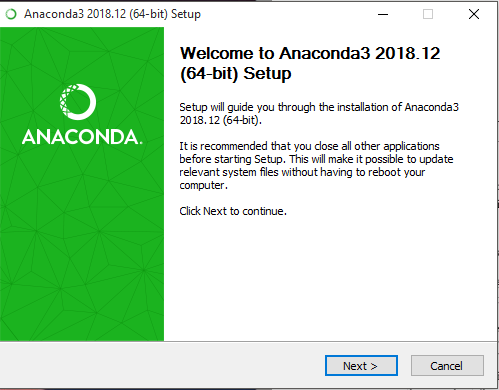
\includegraphics[width=1\textwidth]{figures/fathi/2.PNG}}
\caption{setelah membuka data instalasi klik next}
\label{proses2}

\centerline{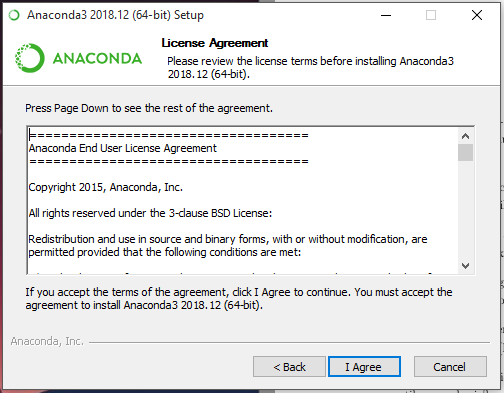
\includegraphics[width=1\textwidth]{figures/fathi/3.PNG}}
\caption{pilih i agree}
\label{proses3}
\end{figure}
\begin{figure}
\centerline{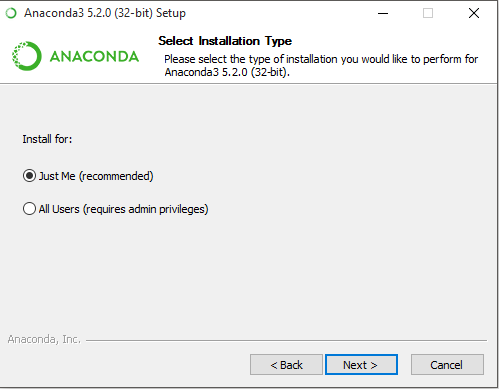
\includegraphics[width=1\textwidth]{figures/fathi/4.PNG}}
\caption{pilih instalasi Just Me}
\label{proses4}

\centerline{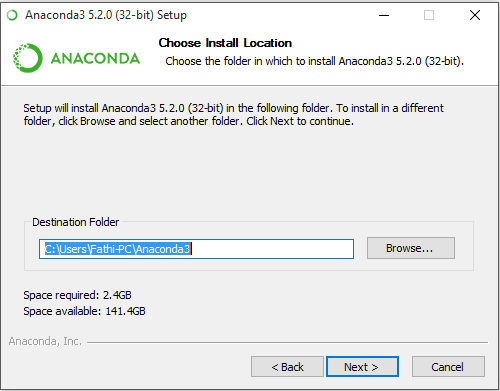
\includegraphics[width=1\textwidth]{figures/fathi/5.PNG}}
\caption{langsung saja next}
\label{proses5}
\end{figure}
\begin{figure}
\centerline{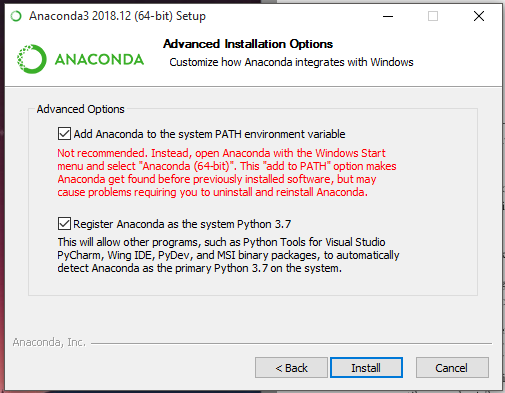
\includegraphics[width=1\textwidth]{figures/fathi/6.PNG}}
\caption{cek kedua pilihan tersebut}
\label{proses6}

\centerline{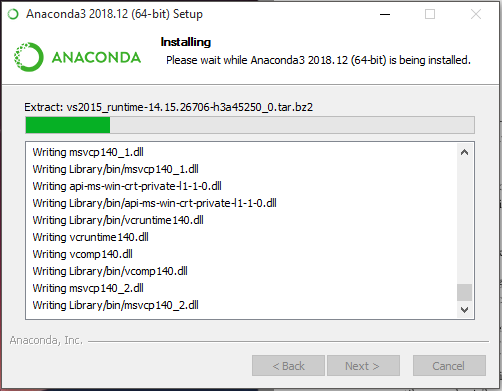
\includegraphics[width=1\textwidth]{figures/fathi/7.PNG}}
\caption{proses Instalasi}
\label{proses7}
\end{figure}
\begin{figure}
\centerline{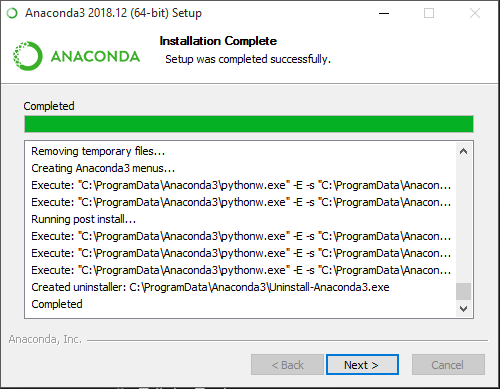
\includegraphics[width=1\textwidth]{figures/fathi/8.PNG}}
\caption{klik next}
\label{proses8}

\centerline{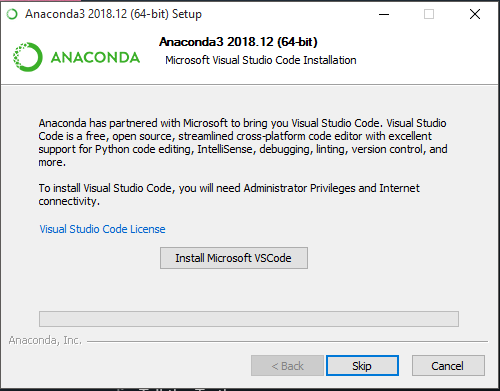
\includegraphics[width=1\textwidth]{figures/fathi/9.PNG}}
\caption{selesai instalasi anaconda}
\label{proses9}
\end{figure}
\begin{figure}
\centerline{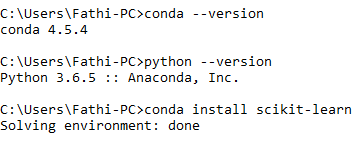
\includegraphics[width=1\textwidth]{figures/fathi/10.PNG}}
\caption{Instalasi SCIKIT dengan menggunakan anaconda}
\label{proses10}

\centerline{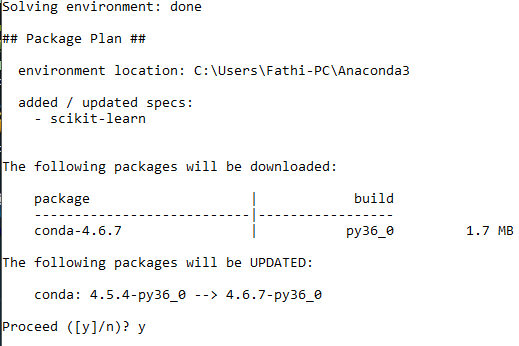
\includegraphics[width=1\textwidth]{figures/fathi/11.PNG}}
\caption{Konfirmasi Instalasi}
\label{proses11}
\end{figure}
\begin{figure}
\centerline{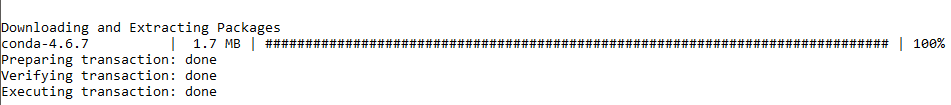
\includegraphics[width=1\textwidth]{figures/fathi/12.PNG}}
\caption{hasil dari instalasi SCIKIT}
\label{proses12}
\centerline{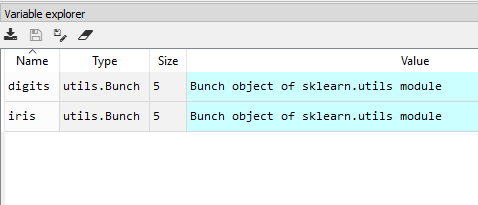
\includegraphics[width=1\textwidth]{figures/fathi/14.PNG}}
\caption{data variable explorer}
\label{proses14}
\end{figure}

\item
Load Example Dataset dan Menjeleaskan kegunakan barisan Code
\subitem
berikut ini adalah contoh dataset yang digunakan untuk melakukan compile ada pada gambar \ref{proses16} dan hasilnya ada pada gambar \ref{proses15}.

\begin{figure}
\centerline{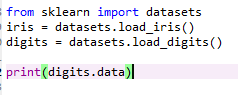
\includegraphics[width=1\textwidth]{figures/fathi/16.PNG}}
\caption{code example dataset yang digunakan}
\label{proses16}

\centerline{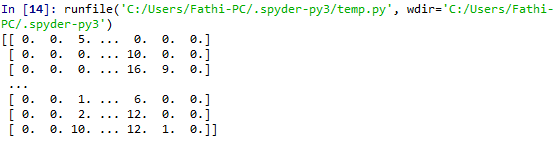
\includegraphics[width=1\textwidth]{figures/fathi/15.PNG}}
\caption{data hasil dari code example dataset yang digunakan}
\label{proses15}
\end{figure}
\begin{itemize}
\item
dari code yang dicoba diketahui bahwa data set yang digunakan adalah data yang diambil dari SKLEARN yang ada pada gambar \ref{proses16}.
\end{itemize}
\begin{itemize}
\item
Learning and Predicting
\subitem
Dalam scikit-learn estimator untuk klasifikasi adalah sebuah objek data python yang memliki implementasi method fit(x, y) dan predict(T). Sebuah estimator danri class sklearn.svm.SVC,yang mana implemetasi dari support vector classification. Estimator dari konstruktor mengambil argument dari model parameter.
\begin{verbatim}
from sklearn import svm
clf = sv.SVC(gamma=0.001, C=100.)
clf.fit(digits.data[:-1], digits.target[:-1]
clf.predict(digits.data[:-1])
\end{verbatim}
\subitem
mengambil nilai data svm ada pada class sklearn, lalu set nilai data dengan clf = sv.SVC(gamma=0.001, C=100.). variable clf digunakan dengan method fit yang di set nilainya [:-1] yang memproduksi array baru dari data digits.data, dengan menggunakan digits.data sebagai acuan, sekarang tinggal melakukan prediksinya.

\item
Model Presistence

\begin{verbatim}
from sklearn import svm
from sklearn import datasets
clf = svm.SVC(gamma=0.001)
iris = datasets.load_iris()
X, y = iris.data, iris.target
clf.fit(X, y)
\end{verbatim}
\subitem
mengambil nilai data svm ada pada class sklearn dan mengambil nilai data datasets ada pada class sklearn, lalu buat variable clf dengan nilai data  dan buat variable yang berisi nilai load\_iris. variable X dan y yang berisi nilai iris data dan iris target, lalu memanggil nilai variable X dan y dengan data variable clf dan method fit.

\begin{verbatim}
import pickle
s = pickle.dumps(clf)
clf2 = pickle.loads(s)
clf2.predict(X[0:1])
y[0]
\end{verbatim}
\subitem
mengambil nilai data pickle dan membuat variable s dengan data nilai pickle.dumps yang berisi data variable clf, membuat variable clf2 dengan data pickle.loads yang menggunakan variable s. menggunakan data variable clf2 dengan method predict dengan data variable X dan data variable y.

\item
Conventions
\begin{itemize}
\item
\begin{verbatim}
import numpy as np
from sklearn import random_projection

rng = np.random.RandomState(0)
X = rng.rand(10, 2000)
X = np.array(X, dtype='float32')
X.dtype

transformer = random_projection.GaussianRandomProjection()
X_new = transformer.fit_transform(X)
X_new.dtype
\end{verbatim}
\subitem
mengambil data numpy dan dialiaskan sebagai np. dari data sklearn mengambil data random\_projection. lalu buat variable rng yang berisi nilai data np dengan random yang berawal 0. lalu variable X dengan data rng yang memiliki type rand berisi data 10 dan 2000. lalu dibuatkan arraynya dengan format X = np.array(X, dtype ='float32'). dan nilai variable transform yang digunakan untuk menampilkan hasil random, dengan format Gaussian random projection. format penampilannya X\_new = transformer.fit\_transform( X) dan X\_new.dtype

\item
\begin{verbatim}
from sklearn import datasets
from sklearn.svm import SVC

iris = datasets.load_iris()
clf = SVC(gamma=0.001)
clf.fit(iris.data, iris.target)

list(clf.predict(iris.data[:3]))

clf.fit(iris.data, iris.target_names[iris.target])

list(clf.predict(iris.data[:3])) 
\end{verbatim}
\subitem
dari data sklearn mengambil datasets dan SVC dari svm, selanjutnya membuat format data variable dengan nilai load\_iris\(\), clf dengan format SVC\(gamma=0.001\), lalu di jalankan dengan moethod clf.fit dengan iris.data dan iris.target sebagai nilainya.

buatkan tampilan datanya dengan list menampilkan data clf dengan predict pada iris.data, dan dilakukan selanjutnya dengan clf.fit dengan nilai data iris.data dan iris.target\_names[ iris.target]. tampilkan lagi dalam bentuk list data tersebut.

\item
\begin{verbatim}
import numpy as np
from sklearn.svm import SVC

rng = np.random.RandomState(0)
X = rng.rand(100, 10)
y = rng.binomial(1, 0.5, 100)
X_test = rng.rand(5, 10)

clf = SVC()
clf.set_params(kernel='linear').fit(X, y)

clf.predict(X_test)

clf.set_params(kernel='rbf', gamma=0.001).fit(X, y)

clf.predict(X_test)
\end{verbatim}
\subitem
mengambil data numpy dan dialiaskan sebagai np dan dari sklearn.svm mengambil data SVC,  lalu buat variable rng yang berisi nilai data np dengan random yang berawal 0, lalu variable X dengan data rng yang memiliki type rand berisi data(100, 10) dan y yang memiliki data (1, 0.5, 100) dengan type data binomial lalu buat X\_test untuk variable test.

\item
\begin{verbatim}
from sklearn.svm import SVC
from sklearn.multiclass import OneVsRestClassifier
from sklearn.preprocessing import LabelBinarizer

X = [[1, 2], [2, 4], [4, 5], [3, 2], [3, 1]]
y = [0, 0, 1, 1, 2]

classif = OneVsRestClassifier(estimator=SVC(gamma=1, random_state=0))

classif.fit(X, y).predict(X)

y = LabelBinarizer().fit_transform(y)
classif.fit(X, y).predict(X)
\end{verbatim}
\subitem
mengambil data sklearn SVC dari svm, OneVsRestClassifier dari multiclass, dan LabelBinarizer dari preprocessing. lalu buatkan variable X dan y yang berisi data nilai dan buatkan data variable classif untuk digunakan sebagai parameter bagi OneVsRestClassfier yang menghitung data estimator SVC. lalu jalankan dengan method fit dan predict, lalu variable y digunakan sebagai parameter yang menjalankan method fit\_transform yang berisi data LabelBinarizer.

\item
\begin{verbatim}
from sklearn.preprocessing import MultiLabelBinarizer
y = [[0, 1], [0, 2], [1, 3], [0, 2, 3], [2, 4]]
y = MultiLabelBinarizer().fit_transform(y)
classif.fit(X, y).predict(X)
\end{verbatim}
\subitem
mengambil data dari sklearn datanya adalah MultiLabelBinarizer dari preprocessing, buatkan variable y ayng berisikan nilai integer untuk di proses agar menghasilkan data seperti berikut
\begin{verbatim}
>>>>>>> c6dbbab89a86daa2bf691a75d9a15c4b56fb15d7
array([[1, 1, 0, 0, 0],
       [1, 0, 1, 0, 0],
       [0, 1, 0, 1, 0],
       [1, 0, 1, 0, 0],
       [1, 0, 1, 0, 0]])
\end{verbatim}
<<<<<<< HEAD
hasil running classif setelah nili parameter y telah di ganti.
\end{itemize}



\subsection{Penanganan Error}\par
\begin{enumerate}
\item
Screenshot Error
untuk lebih jelasnya Screenshot codingan dapat dilihat pada gambar \ref{c5} dan \ref{c6}
\item
Kode error pada screenshot
untuk kode error pada gambar \ref{c5} yaitu pada surce code berikut \begin{verbatim} clf.fit(digits.data[:-1], digits.target[:-1]) \end{verbatim} pada codingan tersebut menjadi error dikarenakan variabel atau method digits belum di definisikan.
sedangkan untuk kode error pada gambar \ref{c6} yaitu pada source code \begin{verbatim} from joblib import dump, load \end{verbatim}  pada codingantersebut terjadi error dikarenakan  module joblib belum di install atau modul tersebut tidak ada di library python.
\item
Solusi Pemecahan Masalah Error 
\begin{itemize}
\item
untuk memperbaiki error pada gambar \ref{c5} tinggal mendefinisikan variabel atau method digits, untuk lebih lengkapnya dapat dilihat pada gambar  \ref{c7} dengan cara tersebut maka masalah error dapat diselesaikan.
\item
sedangkan untuk error joblib bisa dilakukan dengan cara masuk ke cmd administrator kemudian isikan perintah pip install joblib kemudiantekan enter sehingga hasilnya terlihat seperti gambar \ref{c8} setelah itu coba masuk kembali ke python di cmd dan ketikan perintah from joblib import dump, load maka hasilnya seperti gambar \ref{c9}.
\end{itemize}
\end{enumerate}

\begin{figure}[ht]
      \centerline{\includegraphics[width=1\textwidth]
      {figures/c}}
      \caption{Tampilan Versi Python dan Anaconda .}
      \label{c}
      \end{figure}

\begin{figure}[ht]
      \centerline{\includegraphics[width=1\textwidth]
      {figures/c1}}
      \caption{Instalisasi Library Sikic.}
      \label{c1}
      \end{figure}

\begin{figure}[ht]
      \centerline{\includegraphics[width=1\textwidth]
      {figures/c2}}
      \caption{Instalasi Library Sikic Melalui Conda}
      \label{c2}
      \end{figure}

\begin{figure}[ht]
      \centerline{\includegraphics[width=1\textwidth]
      {figures/c3}}
      \caption{Console Python Include Anaconda}
      \label{c3}
      \end{figure}

\begin{figure}[ht]
      \centerline{\includegraphics[width=1\textwidth]
      {figures/c4}}
      \caption{Contoh Codingan Dataset}
      \label{c4}
      \end{figure}

\begin{figure}[ht]
      \centerline{\includegraphics[width=1\textwidth]
      {figures/c5}}
      \caption{Error Coding 1}
      \label{c5}
      \end{figure}

\begin{figure}[ht]
      \centerline{\includegraphics[width=1\textwidth]
      {figures/c6}}
      \caption{Error Coding 2}
      \label{c6}
      \end{figure}


\begin{figure}[ht]
      \centerline{\includegraphics[width=1\textwidth]
      {figures/c7}}
      \caption{Codingan Solusi Untuk Error digits}
      \label{c7}
      \end{figure}

\begin{figure}[ht]
      \centerline{\includegraphics[width=1\textwidth]
      {figures/c8}}
      \caption{Codingan Solusi Untuk Error Joblib}
      \label{c8}
      \end{figure}

\begin{figure}[ht]
      \centerline{\includegraphics[width=1\textwidth]
      {figures/c9}}
      \caption{Hasil Solusi Error Joblib}
      \label{c9}
      \end{figure}
=======
\end{itemize}

\item
Error Handling
\begin{enumerate}
\item
Screenshot
\begin{figure}
\centerline{\includegraphics[width=1\textwidth]{figures/fathi/20.PNG}}
\caption{Error Type data, yang harus digunakan number sedangkan isinya 'SCALE' pada gamma}
\label{proses20}

\centerline{\includegraphics[width=1\textwidth]{figures/fathi/21.PNG}}
\caption{Error no Module found, modul yang dicari tidak ditemukan atau tidak ada 'JOBLIB'}
\label{proses21}
\end{figure}

\item
Error Code and Error Type
\begin{itemize}
\item
Module Not Found
\subitem
module yang dicari tidak ditemukan, karena file yang dicari tidak ada atau belum di instal.

\item
Type Data Error
\subitem
type data yang seharusnya diisikan oleh data number namun diisikan oleh data str/character sedangkan nilai yang bisa dibaca adalah number.
\end{itemize}

\item
Solution
\begin{itemize}
\item
For Module Not Found
\subitem
lakukan instalasi dengan memasukan code berikut untuk download dan instalasi module JOBLIB
\begin{verbatim}
conda install -c anaconda joblib
\end{verbatim}

\item
For Data Type Error
\subitem
ganti isi data menjadi data number, contoh :
\begin{verbatim}
clf = SVC(gamma='scale')
\end{verbatim}
ganti menjadi 
\begin{verbatim}
clf = SVC(gamma=0.5)
\end{verbatim}
\end{itemize}

\end{enumerate}
\end{enumerate}
>>>>>>> c6dbbab89a86daa2bf691a75d9a15c4b56fb15d7
>>>>>>> b1d7802739e393f94f14f567f8e8c88eaba86ce7
